\documentclass[12pt]{article}
\usepackage{verbatim}
\usepackage[dvips]{epsfig}
\usepackage{color}
\usepackage{url}
\usepackage[colorlinks=true]{hyperref}

\begin{document}

\section*{GENESIS: Documentation}

{\bf Related Documentation:}
% start: userdocs-tag-replace-items related-do-nothing
% end: userdocs-tag-replace-items related-do-nothing

\section*{De Schutter: Purkinje Cell Model}

\begin{figure}[h]
\centering
   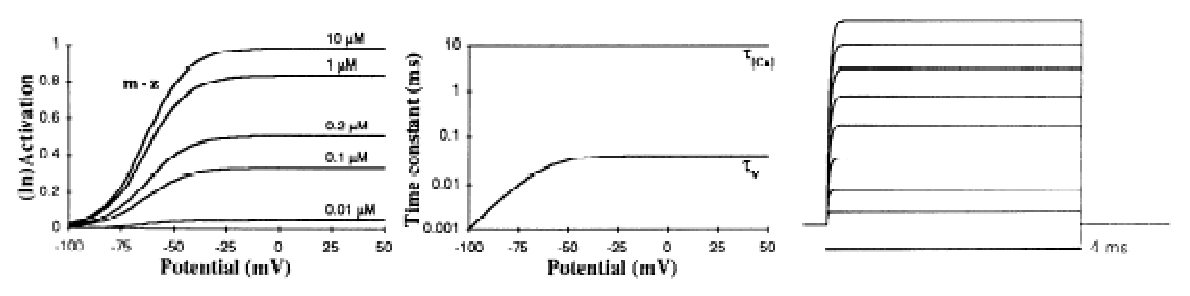
\includegraphics[scale=0.75]{figures/DS1.2H.eps}
   \caption{Activation and inactivation properties of the low-threshold Ca$^{2+}$-activated K$^+$ current (K2, ---) ionic conductances in the model. Seady-state activation and inactivation vs. voltage are plotted at the {\em left}, the time constants of activation ($\tau_m$) and inactivation ($\tau_h$) vs. voltage in the {\em middle} (Note: Semilogarithmic scale), and a simulation of representative voltage-clamp currents at the {\em right}. Note: Activation is controlled by the product of a voltage and a [Ca$^{2+}$]-dependent factor, each with their own time constants ($\tau_v$ and $\tau_{[Ca]}$). The voltage clamps simulate steps from a holding potential of -110 to -70\,mV up to 0\,mV in 10\,mV increments. The voltage-clamp current amplitude has been scaled arbitrarily because we mainly wanted to demonstrate the current kinetics.}
   \label{fig:DS1.2H}
\end{figure}

\subsection*{Low-threshold Ca$^{2+}$-activated K$^+$ (K2) Current}

In their single-channel study of K$^+$ channels in Purkinje cells,\,\cite{Gruol:1991dz} describe 2 Ca$^{2+}$-activated K$^+$ channels. One is a 134\,pS (symmetrical K$^+$ conditions) channel, which they identify as the K2 channel. These authors report that this channel composes $\sim$\,13\,\% of the total Ca$^{2+}$-activated K$^+$ conductance, activates at lower potentials than the BK channel, and is blocked by TEA. However,\,\cite{Gruol:1991dz} does not contain enough data to model this channel. The K2 channel is not a small K channel (SK) channel, because SK channels have a lower slope conductance (10--20\,pS), are not voltage sensitive\,\cite{Lancaster:1991ye, Lang:1987qo} and are blocked by apamin\,\cite{Latorre:1989fu}. In rat brain synaptosomal membranes several types of Ca$^{2+}$-activated K$^+$ channels have been characterized, some of which have a medium-sized conductance, are TEA-sensitive, and are not blocked by apamin. A 110- to 125\,pS channel described by\,\cite{Farley:1988tw} is sensitive to low concentrations of Ca$^{2+}$, so that most of the channels are open at 0.1\,$\mu$M, is activated by 30\,mV depolarizations, and is blocked by charybdotoxin and by high concentrations of TEA. A 135\,pS channel described by\,\cite{Reinhart1989:xe} is sensitive to submicromolar concentrations of Ca$^{2+}$, has a Hill coefficient of $\sim$\,2, has several closed states, has faster kinetics than the BK channel, and is blocked by charybdotoxin.

Because we did not have enough data available to describe the K2 channel completely, we used the same kinetic scheme as for the BK channel but with a lower voltage threshold, faster kinetics, and a lower half-activation Ca$^{2+}$ concentration of 0.2\,$\mu$M. Thus, despite the similar form of the equations, the K2 channel is quite different from the KC channel in voltage- and Ca$^{2+}$ dependence.

\bibliographystyle{plain}
\bibliography{../tex/bib/g3-refs}

\end{document}
